\chapter{ Metodologia}\label{meto}

A metodologia utilizada é um modelo preditivo de Suporte a Decisão que forneça informação suficiente a um gestor para decidir quando e por onde 
enviar uma frota de caminhões por determinada rodovia que apresente retenções crescentes de logística de cargas. As soluções disponíveis que 
existem tais como; Google Maps, Waze e outros dessa natureza somente exibem informações momentâneas, produzidas e compartilhadas pelos utilizadores 
dos aplicativos ou por informações provindas de GPS, contudo não analisam dados históricos dessas rodovias nem fazem predições futuras sobre o 
comportamento delas. \\

\section{ Plano geral da metodologia}

Propomos um plano que contemple 3 etapas, cada uma dividida em fases atinentes. A figura a seguir ilustra essa metodologia descrita graficamente, onde as três etapas são representadas por retângulos.
 
\begin{figure}[ht]
\centering
\caption{Etapas da gerais da metodologia}
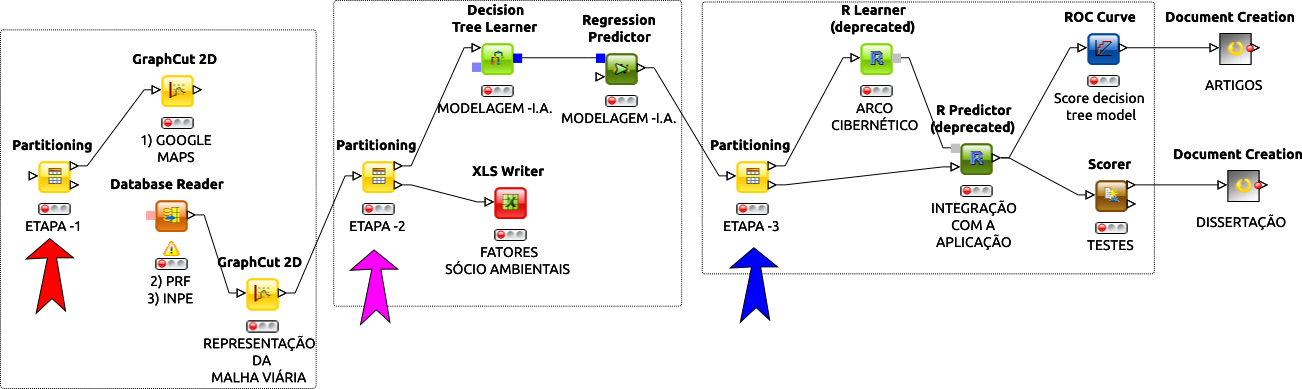
\includegraphics[width=160mm, height=70mm]{Figuras/BigData/Etapas.png}
\end{figure}

 A etapa 1 contempla as fases da coleta das bases vetoriais, das bases de dados históricas e proposição de um modelo de representação único.
 
 O retângulo central é a etapa 2, que consiste nas fases de Identificação dos fatores sócio ambientais na bases históricas, a modelagem do sistema preditivo e aplicação das técnicas de IA. Propomos inicialmente a Regressão Logística e Árvores de decisão, testes iniciais e depuração do modelo.
 
 A última etapa da nossa proposta metodológica é a etapa 3, esta conterá um arco cibernético construído com os dados de redes sociais, como por exemplo a API do Twitter, este ``per si'' fará com que o modelo preditivo seja retro-alimentado, 
 mantendo-o, ao longo do tempo atualizado na perspectiva do usuário gestor. Isso pois, modelos preditivos com o passar do tempo tendem a desfasar-se. 
 Uma proposta algorítmica para substituir a API das redes sociais 
 poderá ser desenvolvida e testada numa fase complementar, o algorítmo Ant-Miner poderá vir a ser um candidato de adaptação.\\
 
 A representação da malha viária que acopla a estrutura dinâmica com a outra estrutura será o ``front-end'' da metodologia proposta estará na 
 terceira etapa.


\section{ Proposição do modelo preditivo}

O modelo preditivo foi construído utilizando bases de dados históricas da PRF (de acidentes e de paralisações ex: protestos) entre Janeiro de 2007 a 
Dezembro 2015. As bases de dados do Batalhão de Polícia de Rodoviária estadual -- BPRv vieram entre Janeiro/2010 a Julho/2016, cortes em ambas as bases foram 
feitos para adequar as datas. Essas bases de dados são integradas gerando um único e complexo modelo preditivo que será acoplado a estrutura dinâmica.


%\pagebreak

\section{ Reflexão sobre as tecnologias utilizadas no modelo preditivo}\label{result}

Não existe uma técnica de mineração que generalize os mais diversos ambientes preditivos, mas sim um ``pool'' dessas técnicas onde uma complementa outra.
As técnicas preditivas tradicionais que contemplam análise de grandes massas de dados como base heterogêneas são possíveis quando adaptadas para uma forma comparável à que
foram inicialmente concebidas, por que as variáveis em uma base de dados a priori guardam pouca relação as variáveis de outra base de dados.
neste caso essas variáveis ou são excluídas ou são transformadas a fim de ``guardarem'' um correlação com a outra base de dados. 
Quando há uma proximidade entre as bases de dados, na fase de transformação de dados, onde são criadas novas variáveis, a proximidade entre as
bases se estreita. 
Nesta pesquisa, bases heterogêneas foram integralizadas num única grande base, onde as variáveis independentes foram
em sua maioria preservadas e/ou construídas novas, nas bases onde não haviam correspondência, respeitando a lógica do negócio.\\
A tabela a seguir descreve as variáveis originais na base de dados de acidentes da PRF 


\subsection{ Metodologia utilizada para coleta dos dados}\label{intro:metodologia}


As informações para suprir nosso modelo preditivo estão disponíveis na Internet, em sua maioria são Dados Governamentais Abertos, tais como os dados
da PRF, INPE e IBGE. Isto são iniciativas governamentais para fomentar a participação popular, dentro outros motivos, essas informações são também 
conhecidas como \textit{open data} \cite{DadosGoverno}, contudo os dados referentes à PRF e ao BPRv, para esta pesquisa, foram cedidos pelos respectivos 
órgãos governamentais (ver anexos) já em formato CSV para serem utilizados exclusivamente nesta pesquisa. Isso possibilitou ganho qualitativo nos dados evitando 
passar pelos transtornos como descreve Costa (2015) quando coletou os dados diretamente da Internet.\cite{Costa2015} 
As bases de dados do INPE e do base de dados do IBGE apresentaram boa qualidade o que justificou serem serem coletados diretamente da Internet.


\begin{table}[htbp!]
 \centering
  \caption{Variáveis originais da base de acidentes} 
  \begin{tabular}{r|l} \hline
   Ano & Ano da ocorrência do acidente\\
   Mês & Mês de ocorrência do acidente\\
   Num & Número do mês do acidente ex: 1 = Janeiro \\
   KM & Numeração do quilômetro \\
   BR & Numeração da Br\\
   Latitude & Latitude da ocorrência \\
   Longitude & Longitude da ocorrência \\
   Condição Pista & Condição da pista: seca, molhado, ... \\
   Restrição de Visibilidade & Restrição de visibilidade: inexistente, neblina, .., outros \\
   Tipo Acidente & Tipo de Acidente: atropelamento, colisão lateral,..\\
   Cauda Acidente & A possível causa do acidente: Falta de atenção, ... \\
   Sentido Via & Sentido da via: crescente, decrescente \\
   Traçado Via & Tipo de traçado da via: reta, curva, cruzamento, ... \\
   Município  & Localidade onde ocorreu \\
   Tipo veículo & Tipo de veículo envolvido no acidente \\
   Data Inversa & Data do acidente no formato dd/mm/aa \\
   Horário & Hora que ocorreu o acidente no formato hh/mm/ss \\
   Qtd Feridos Graves & Quantidade de feridos graves envolvidos \\
   Qtd Feridos Leves & Quantidade de feridos leves envolvidos\\
   Qtd Ilesos & Quantidade de ilesos envolvidos\\
   Qtd Mortos & Quantidade de mortos envolvidos \\
   Qtd Pessoas & Quantidade de pessoas envolvidos \\
   Qtd Veículos & Quantidade de veículos envolvidos\\
   Qtd Acidentes Graves & Quantidade de acidentes graves \\
   Qtd Ocorrências & Quantidade de ocorrências \\
  \end{tabular}
\end{table}

\pagebreak

Na tabela seguinte; as variáveis originais da base de dados da PRF com interdições das vias 
(somente interdições que paralisaram as BRs, não contém acidentes, exemplo: passeatas, protestos) 

\begin{table}[htbp]
 \centering
  \caption{Variáveis originais da base de interdições}
  
  \begin{tabular}{r|l} \hline
   Comunicação & Código do agente que comunicou o incidente \\
   Data Hora & Data hora no formato dd/mm/aa mm:ss \\
   BR & Numeração da Br do incidente\\
   KM & Numeração do quilômetro do incidente\\
   Trecho  & Local onde ocorreu o incidente \\
  \end{tabular}
\end{table}



\subsection{ As variáveis do modelo preditivo}

Algumas técnicas de IA são altamente sensíveis a dados ausentes os ``missing data'' à dados com pouca consistência e outros tipos de dados 
comuns em bases mantidas sem um bom critério de inserção dos dados. 
A variável dependente foi designada como \textbf{gargalo} e as variáveis independentes (ou explicativas) são:


\begin{table}[htbp]
 \centering
  \caption{Variáveis do modelo preditivo}
  
  \begin{tabular}{r|l} \hline
   KM & Numeração do quilômetro \\
   BR & Numeração da Br\\
   condPista & Condição da pista: seca, molhado, ... \\
   restVisibili & Restrição de visibilidade: inexistente, neblina, .., outros \\
   tipoAcident & Tipo de Acidente: atropelamento, colisão, paralisação,...\\
   tipoDano  & Tipo de Dano: leve, médio, grave \\
   Municipio  & Localidade onde ocorreu \\
   Ano & Ano que ocorreu o acidente \\
   Mês & Mês que ocorreu o acidente \\
   Dia & Dia que ocorreu o acidente \\
   Hora & Hora que ocorreu o acidente \\
  \end{tabular}
\end{table}



 
À base de dados da PRF, relativas a interdições das vias, por motivos diversos, não haviam variáveis tais como; visibilidade, condições da via, gravidade paralisação e outras.
Foram incorporadas à essa base essas novas variáveis, para populá-las, adotou-se a lógica; presumivelmente protestos são realizados com boa visibilidade, em condições de via razoáveis e a gravidade da paralisação foi considerada leve.

As técnicas como Redes Neurais Artificias (MLP) [\large{CITAR}], Árvores de decisão (CART) [\large{CITAR}], Regressão logística (MLR) 
[\large{CITAR}] fornecem visão generalizada dos fatores preponderantes, levantando padrões ocultos nos dados. Esta fase é conhecida como 
Aprendizagem de Máquina (acrônimo de Machine Learning)

\begin{itemize}
 \item[a] Redes Neurais Artificias do tipo \textit{ Multi Layer Perceptron}  -- (MLP) têm capacidade de receber várias entradas ao mesmo tempo e distribuí-las de maneira organizada, além 
	  são simples de implementar e trazem resultados satisfatórios em grandes bases de dados.
 
 \item[b] Árvores de decisão para classificar acidentes do tipo \textit{ Classification and Regression Tree}  -- (CART) foi empregue por Pakgohar et al no artigo 
	  \textit{The role of human factor in incident and severity of road crashes based on the CART and LR regression a data mining approach}  com nível de acurácia próximo aos 80\%

 \item[c] Regressão logística tipo \textit{Multinomial Logistic Regression} -- (MLR) fornece a possibilidade de aprofundamento em vários níveis de busca sendo a mais apropriada, já que Regressão logística 
	  tradicional não permite aprofundamento desse tipo no espaço de busca.
\end{itemize}



\begin{figure}[ht]
  \centering
    \caption{Etapas 1 -- Coleta e união das bases históricas de acidentes e interdições}
    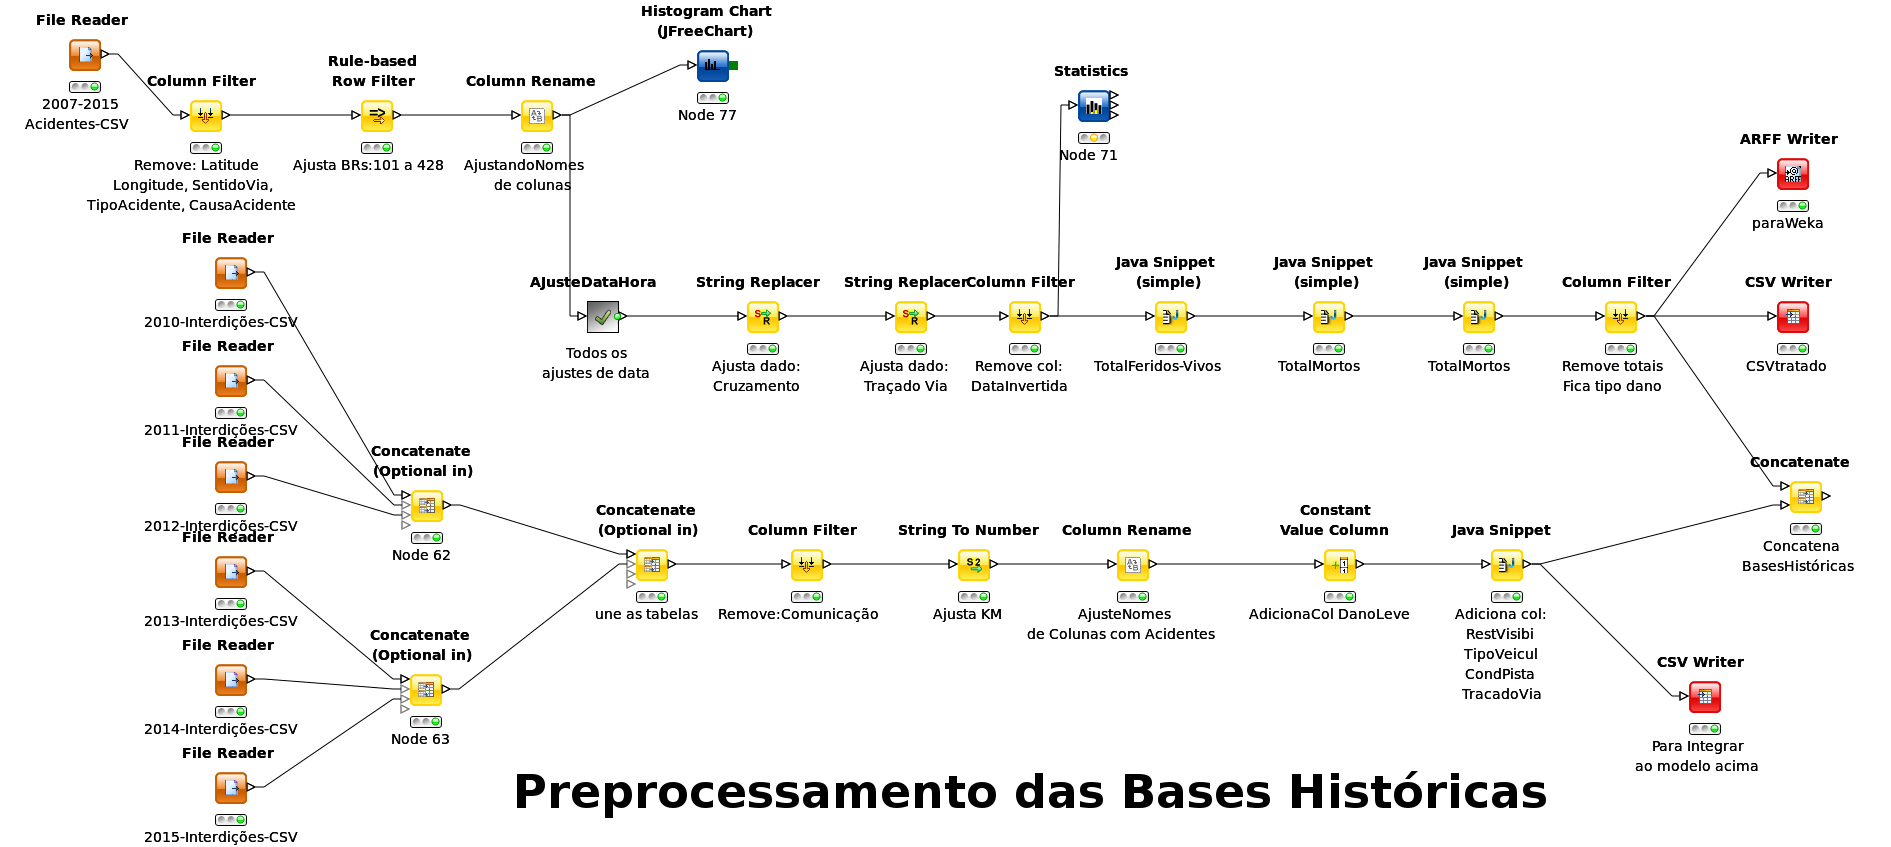
\includegraphics[width=165mm, height=100mm]{Figuras/Cronograma/BasesHistoricas.png}
\end{figure}

\section{ Extração do conhecimento}

\pagebreak

\section{ Acoplamento com a estrutura dinâmica}

A estrutura dinâmica é composta por duas API's, uma disponibilizada pela Google, através do Google Maps que está atualmente na versão V3 e 
outra uma API do Twitter. A API do Google Maps proporciona uma ``leitura'' atualizada em forma de mapa no momento em que a estrutura dinâmica ``roda''. 

A API do Twitter também tem a possibilidade de atualizar o modelo preditivo, contudo o objetivo desta é faz um Arco cibernético, 
retroalimentando todo o sistema com novas informações, pensamos que isso permite que o primeiro módulo (preditivo) seja atualizado de 
tempos em tempos, quando for .

A API Google Maps portanto é o ``front-end'' do Sistema e uma futura aplicação que poderá ser desenvolvida para ser executada em um aparelho 
celular, ``Smartphones'', com capacidade para executar aplicativos mais complexos.


\begin{figure}[ht]
\centering
\caption{Etapas da metodologia}
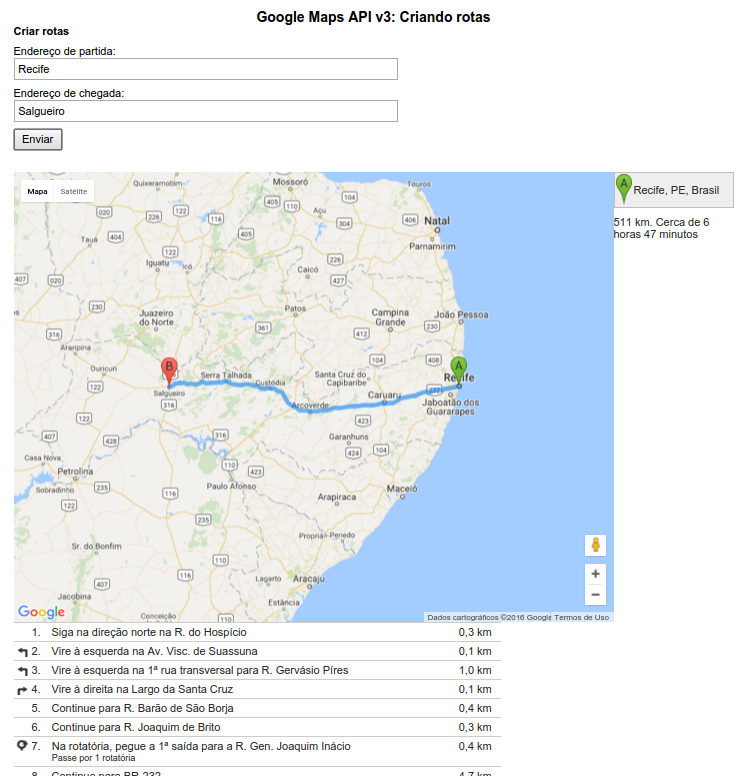
\includegraphics[width=150mm, height=130mm]{Figuras/Cronograma/GoogleMaps.png}
\end{figure}
 

Concluída as três etapas e com as informações geradas pelo modelo serão escritos artigos científicos  pertinentes à pesquisa em lide e a escrita da dissertação.
 
 
 
\pagebreak 
 
\section{Cronograma}\label{intro:cronograma}


\begin{table}[htbp]
 \scriptsize
      \centering  \caption{Cronograma -- 12 meses}
	\begin{tabular}{l|c|c|c|c|c|c|c|c|c|c|c|c}
	\hline
	\textbf{Etapas/2016} & \textbf{Fev} & \textbf{Mar} & \textbf{Abr} & \textbf{Mai}& \textbf{Jun} & \textbf{Jul} & \textbf{Ago} & \textbf{Set} & \textbf{Out} & \textbf{Nov} & \textbf{Dez} & \textbf{Jan/17} \\
	  \hline
	  Rev. da literatura. & x & x & x & x & x & x & x & --- & --- & --- & --- & --- \\ \hline
	  Etapa -- 1 & x & x & x & --- & --- & --- & --- & --- & --- & --- & --- & --- \\ \hline
	  Etapa -- 2 & --- & --- & --- & x & x & x & --- & --- & --- & --- & --- & --- \\ \hline
	  Etapa -- 3 & --- & --- & --- & --- & --- & --- & x & x & x & --- & --- & --- \\ \hline
	  Escrita de artigos & --- & --- & --- & --- & --- & --- & --- & --- & x & x & x & --- \\ \hline
	  Escrita da dissertação & --- & --- & --- & --- & --- & --- & --- & --- & x & x & x & --- \\ \hline
	  Defesa & --- & --- & --- & --- & --- & --- & --- & --- & --- & --- & --- & x \\ \hline
	\end{tabular}
\end{table}


 



